
\sujet{Geometry}

\noindent
{\bf Duration: 1h30 / 20 points\\}

\begin{note}For each exercise, you can propose several approaches to address the issue. At the end of the exam, you will send the source codes (with comments!) by email to the following address: \texttt{debayle@emse.fr}.
\vspace{.5cm}

All paper documents are allowed, connection to campus website is allowed. All other internet connection if forbidden.\end{note}

\section{Granulométrie (10 points)}
The following 2-D image represents a set of discs whose grain size (size distribution) has to be determined. %La difficulté réside dans la connectivité de certains disques. En effet, certaines composantes connexes représentent des amas de plusieurs disques connectés, que nous souhaitons donc  individualiser pour faciliter la caractérisation. 
\begin{figure}[h]
\begin{center}
{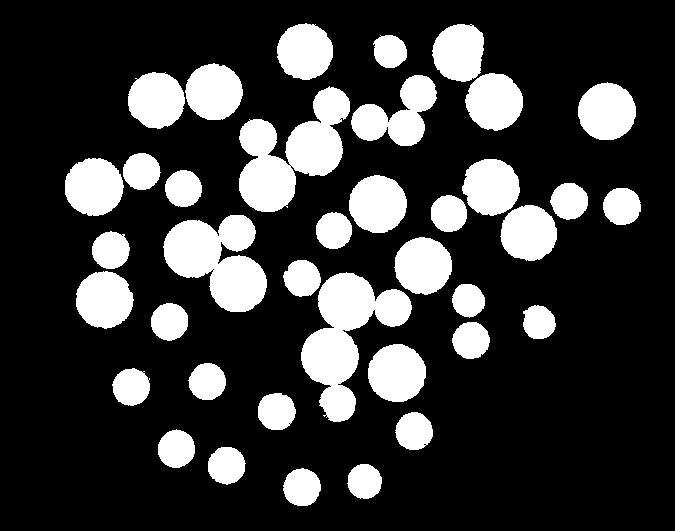
\includegraphics[width=5cm]{disks.png}}
\end{center}
\end{figure}

\begin{qbox}
\begin{itemize}
\item Set up a procedure to determine the number of disks.
\item Let us consider that this disk population is composed of two size classes. Determine the number of discs for each class.
\end{itemize}
\end{qbox}

\section{Geometric covariogram (10 points)}
The geometric covariogram of a convex set $K\subseteq \mathbb{R}^2$ is defined by the following application:
\begin{eqnarray}
\gamma_K(u)=A(K\cap (K+u))
\end{eqnarray} 
where $u$ is a vector of $\mathbb{R}^2$ and $A$ is the area measure.\\
The following figure illustrates the covariogram of a rectangle $K$ for a certain vector $u$ :
\begin{figure}[h]
\centering
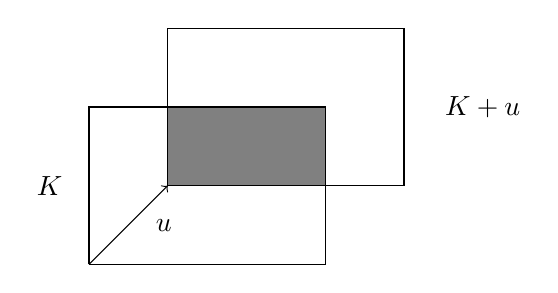
\begin{tikzpicture}
\draw[] (0,0)--(3,0)--(3,2)--(0,2)--(0,0);
\draw[] (1,1)--(4,1)--(4,3)--(1,3)--(1,1);
\draw[fill=gray] (1,1)--(3,1)--(3,2)--(1,2)--(1,1);
\draw[->] (0,0)--(1,1);
\node at (0.95, 0.5) {$u$};
\node at (-0.5, 1) {$K$};
\node at (5, 2) {$K+u$};
\end{tikzpicture}
\end{figure}

\noindent Often we are interested in the isotropic covariogram $\overline{\gamma}_K(r), r\in \mathbb{R}$ as the average of $\gamma_K(ru)$ on all possible directions $u\in S^1$ (uniform distribution on the disc $S^1$).\\
Although it is often difficult to obtain an explicit formula for $\overline{\gamma}_K(r)$, one have analytical expression for some elementary sets K. For example, for a disc with a radius of $R$, its isotropized covariogram is given by:
\begin{eqnarray}
\overline{\gamma}_K(r)=2R^2\cos^{-1}\left(\frac{r}{2R}\right)-\frac{\sqrt{4R^2-r^2}}{2}, \textrm{ pour } 0\leq r \leq 2R \label{eq:cov_disc}
\end{eqnarray}

\begin{qbox}
\begin{itemize}
\item Simulate a disc with a radius of $R$ and numerically calculate its isotropic covariogram. Notice that \minline{meshgrid} could be useful to generate a binary image of a disc.
\item Compare your estimated covariogram with the analytical covariogram via Eq.\ref{eq:cov_disc}.
\item By repeating this procedure for discs of different radii, plot the relative error between the two covariograms (estimated and analytical) as a function of the $R$ radius of the disc.
\end{itemize}
\end{qbox}

